\newpage
\section{Projektowanie}

\subsection{Wykorzystywane narzędzia i technologie}

Projekt został opracowany w języku C++, który umożliwia tworzenie
struktur danych oraz zarządzanie pamięcią dynamiczną. Program
realizuje działanie listy dwukierunkowej przechowującej elementy
w pamięci sterty.

Podczas realizacji projektu wykorzystywane są następujące narzędzia:

\begin{itemize}
    \item \textbf{C++} -- język programowania wykorzystany do
    implementacji listy dwukierunkowej oraz wzorców projektowych.

    \item \textbf{Kompilator C++} -- narzędzie służące do
    przekształcania kodu źródłowego w program wykonywalny.

    \item \textbf{Git} -- system kontroli wersji umożliwiający
    śledzenie zmian w kodzie, tworzenie commitów oraz przywracanie
    wcześniejszych wersji projektu.

    \item \textbf{GitHub} -- platforma umożliwiająca
    przechowywanie repozytorium zdalnego, synchronizowanie zmian
    oraz pobieranie projektu w różnych lokalizacjach.

    \item \textbf{Doxygen} -- narzędzie automatycznie generujące
    dokumentację na podstawie komentarzy i struktury kodu źródłowego.

    \item \textbf{LaTeX} -- system składu tekstu wykorzystywany do
    przygotowania dokumentacji projektowej oraz wygenerowania
    dokumentacji w formacie PDF.
\end{itemize}

\subsection{Struktura projektu}

Projekt został podzielony na osobne pliki, aby oddzielić
odpowiedzialności poszczególnych klas. Ułatwia to rozwijanie
programu, testowanie jego działania oraz utrzymanie kodu.

W projekcie wykorzystywane są następujące klasy i pliki:

\begin{itemize}
    \item \textbf{Node} -- reprezentuje pojedynczy węzeł listy.
    Przechowuje wartość elementu oraz odwołania do poprzedniego
    i następnego węzła.

    \item \textbf{NodeFactory} -- odpowiada za tworzenie nowych
    węzłów. Zastosowanie wzorca Factory oddziela proces tworzenia
    obiektów od pozostałej logiki programu.

    \item \textbf{Iterator} -- umożliwia przechodzenie po elementach
    listy oraz obsługę operacji związanych z odczytem kolejnych
    i poprzednich elementów.

    \item \textbf{List} -- implementuje listę dwukierunkową.
    Przechowuje wskaźniki na pierwszy i ostatni element oraz
    informacje o liczbie elementów. Udostępnia metody dodawania,
    usuwania, wyświetlania i czyszczenia listy.

    \item \textbf{main} -- zawiera funkcję główną programu,
    w której tworzony jest obiekt listy i testowane są
    dostępne operacje.
\end{itemize}

\subsection{Zastosowane wzorce projektowe}

\subsubsection{Wzorzec Factory}

Wzorzec Factory został zastosowany do tworzenia węzłów listy.
Zamiast umieszczać całą logikę tworzenia obiektów bezpośrednio
w klasie \texttt{List}, program korzysta z klasy
\texttt{NodeFactory} i jej metody \texttt{create()}.

Takie rozwiązanie oddziela tworzenie węzłów od operacji
wykonywanych na liście. Ułatwia również modyfikowanie sposobu
tworzenia obiektów w przyszłości.

\subsubsection{Wzorzec Iterator}

Wzorzec Iterator służy do poruszania się po elementach listy.
Umożliwia odczytywanie kolejnych elementów oraz przechodzenie
do elementu poprzedniego bez konieczności umieszczania całej
logiki iteracji w klasie głównej programu.

W połączeniu z listą dwukierunkową pozwala to na obsługę
przechodzenia w obu kierunkach.

\subsection{Zarządzanie pamięcią}

Elementy listy są tworzone dynamicznie w pamięci sterty.
Każdy węzeł przechowuje wartość oraz dwa odwołania:
do poprzedniego i następnego elementu.

Podczas dodawania elementu należy odpowiednio zaktualizować
powiązania między węzłami. Przy usuwaniu elementu konieczne
jest zachowanie poprawności połączeń pozostałych węzłów
oraz zwolnienie pamięci zajmowanej przez usuwany obiekt.

Szczególną uwagę należy zwrócić na przypadki, w których lista
jest pusta lub zawiera tylko jeden element. Metoda
\texttt{clear()} powinna usuwać wszystkie elementy listy
i przywracać jej stan początkowy.

\subsection{Konfiguracja kompilatora}

Kod źródłowy jest kompilowany za pomocą kompilatora zgodnego
z językiem C++. Podczas kompilacji należy uwzględnić wszystkie
pliki źródłowe zawierające implementacje klas oraz plik
z funkcją \texttt{main()}.

Przykładowe polecenie kompilacji z wykorzystaniem kompilatora
\texttt{g++} przedstawiono poniżej:

\begin{verbatim}
g++ -std=c++17 -Wall -Wextra -pedantic \
    main.cpp List.cpp Node.cpp NodeFactory.cpp Iterator.cpp \
    -o PZ_Projekt_Listy
\end{verbatim}

Parametry kompilacji oznaczają:

\begin{itemize}
    \item \texttt{-std=c++17} -- wykorzystanie standardu C++17,
    \item \texttt{-Wall} -- włączenie wielu ostrzeżeń kompilatora,
    \item \texttt{-Wextra} -- włączenie dodatkowych ostrzeżeń,
    \item \texttt{-pedantic} -- zgłaszanie problemów związanych
    z niezgodnością ze standardem języka,
    \item \texttt{-o PZ\_Projekt\_Listy} -- określenie nazwy
    pliku wynikowego.
\end{itemize}

Podane polecenie przedstawia przykładową konfigurację kompilacji.
Nazwy plików oraz standard języka należy dopasować do faktycznej
struktury projektu i używanego środowiska.

\subsection{Biblioteki}

Projekt może korzystać ze standardowych bibliotek języka C++,
w zależności od zastosowanych instrukcji i sposobu wyświetlania
wyników. Nie jest wymagane wykorzystywanie zewnętrznych bibliotek
do samej implementacji listy dwukierunkowej.

W przypadku korzystania z biblioteki standardowej jej nagłówki
należy dołączać w plikach, w których są potrzebne. Przykładowo
biblioteka \texttt{<iostream>} umożliwia obsługę wejścia i wyjścia,
natomiast \texttt{<cstddef>} udostępnia między innymi typ
\texttt{std::size\_t}.

\subsection{Diagram zależności klas}

Poniższy schemat przedstawia najważniejsze klasy projektu
i ich zależności.

\begin{figure}[H]
    \centering
    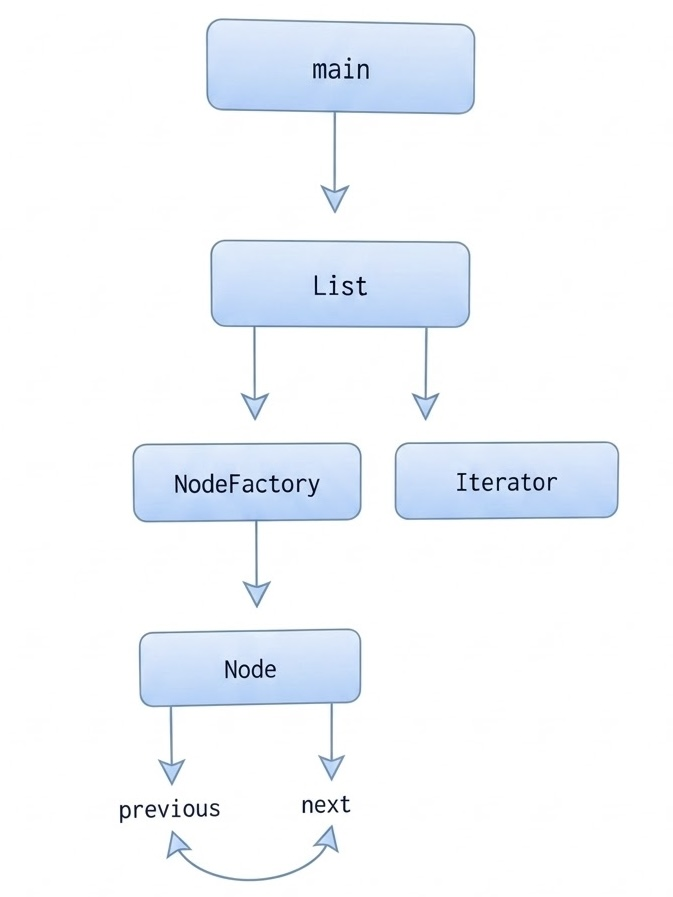
\includegraphics[width=0.8\textwidth]{rys/diagram.jpg}
    \caption{Diagram zależności klas projektu}
    \label{fig:diagram-zaleznosci}
\end{figure}

Klasa \texttt{List} odpowiada za organizację elementów
i udostępnianie operacji na liście. \texttt{NodeFactory}
uczestniczy w tworzeniu węzłów, a \texttt{Iterator}
umożliwia poruszanie się po elementach. Węzły klasy
\texttt{Node} są połączone w obu kierunkach.

\subsection{Schemat działania programu}

Działanie programu można przedstawić w następujących krokach:

\begin{enumerate}
    \item Uruchomienie programu w funkcji \texttt{main()}.
    \item Utworzenie obiektu listy dwukierunkowej.
    \item Wykonanie wybranych operacji na liście.
    \item W razie dodawania elementu utworzenie nowego węzła
    i połączenie go z odpowiednimi elementami.
    \item W razie usuwania elementu aktualizacja połączeń
    oraz zwolnienie pamięci.
    \item Wyświetlenie listy w kolejności od początku do końca
    lub od końca do początku.
    \item Sprawdzenie działania iteratora przez przechodzenie
    do następnych i poprzednich elementów.
    \item Usunięcie wszystkich elementów i zakończenie programu.
\end{enumerate}

\subsection{Kontrola wersji za pomocą Git i GitHub}

Podczas realizacji projektu wykorzystywany jest system Git,
który pozwala zapisywać kolejne etapy pracy nad programem.
Każdy commit reprezentuje zapis zmian wprowadzonych w kodzie
źródłowym.

Repozytorium GitHub umożliwia przechowywanie kopii projektu
na serwerze oraz synchronizowanie zmian pomiędzy różnymi
lokalizacjami. Dzięki temu można kontynuować pracę na pobranej
kopii projektu, przesyłać zmiany do repozytorium zdalnego
i pobierać aktualizacje do pozostałych kopii.

W ramach projektu Git służy również do sprawdzania działania
operacji związanych z historią zmian, w tym przywracania
wcześniejszych wersji oraz usuwania wybranych commitów.
Pozwala to przeanalizować wpływ zmian w kodzie na poprawność
kompilacji programu.

\subsection{Generowanie dokumentacji za pomocą Doxygen}

Doxygen jest wykorzystywany do automatycznego generowania
dokumentacji na podstawie kodu źródłowego oraz komentarzy.
Plik konfiguracyjny \texttt{Doxyfile} określa między innymi
formaty dokumentacji i katalog wyjściowy.

W projekcie włączono generowanie dokumentacji HTML oraz LaTeX.
Wygenerowane pliki LaTeX mogą następnie zostać skompilowane
do dokumentu PDF.

Podstawowy proces generowania dokumentacji obejmuje:

\begin{enumerate}
    \item Przygotowanie i uzupełnienie pliku \texttt{Doxyfile}.
    \item Uruchomienie programu Doxygen.
    \item Wygenerowanie plików dokumentacji.
    \item Przejście do katalogu zawierającego pliki LaTeX.
    \item Skompilowanie dokumentacji do formatu PDF.
\end{enumerate}

Automatyczne generowanie dokumentacji ułatwia przedstawienie
struktury projektu, klas, metod i zależności pomiędzy
poszczególnymi elementami programu.